\documentclass{standalone}
\usepackage{tikz}
\usetikzlibrary{patterns, positioning}

\begin{document}
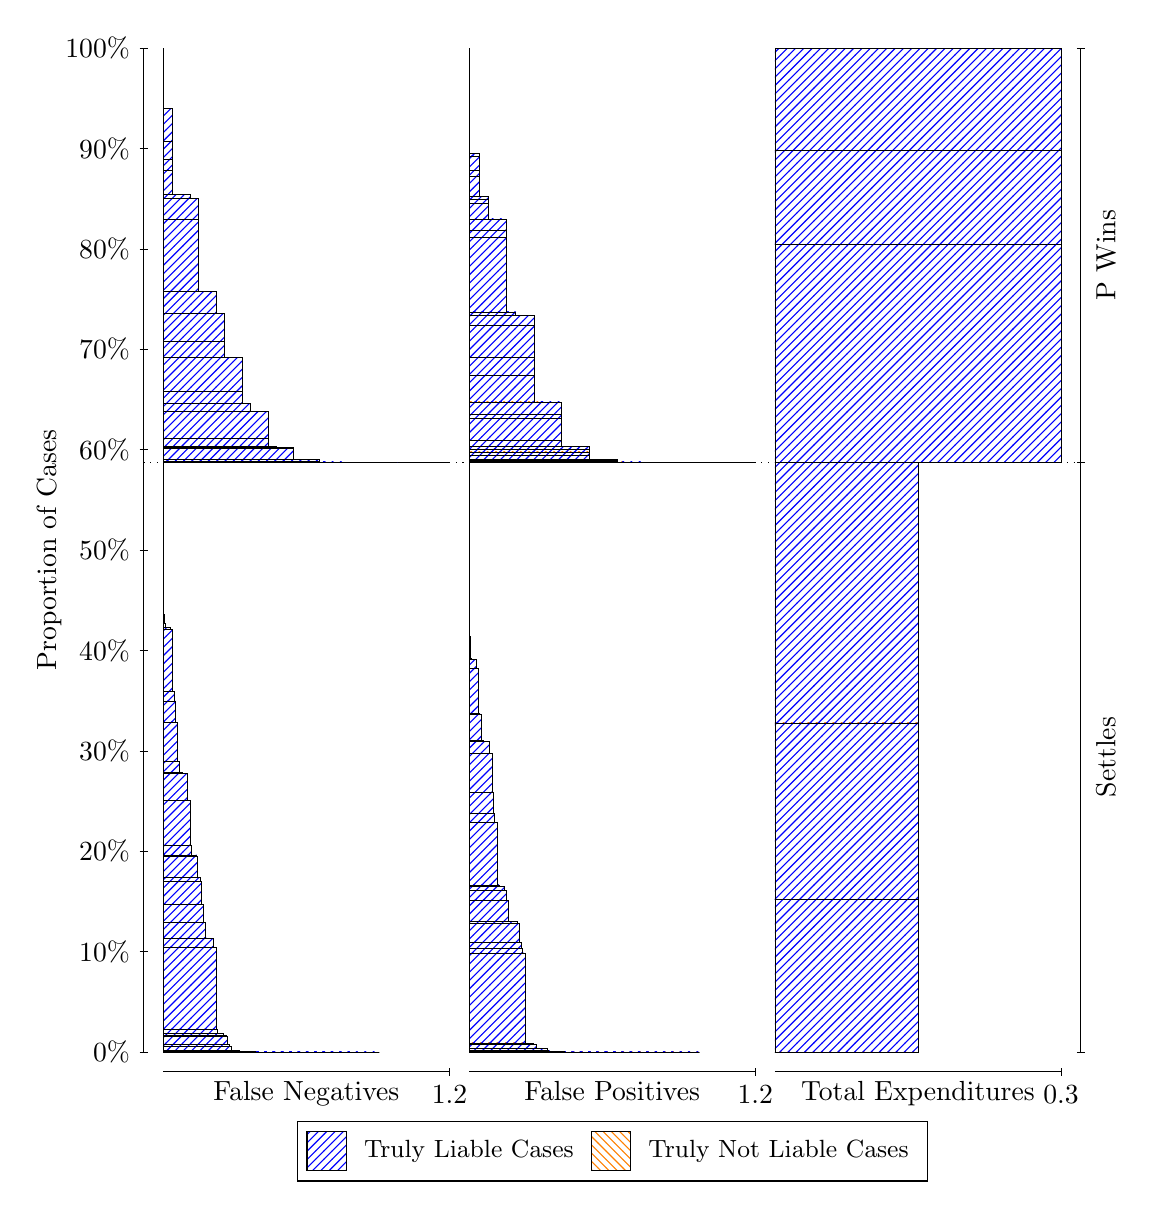
\begin{tikzpicture}
\draw[black, very thin] (1.5,1.75) -- (1.5,14.5);
\node[rotate=90, anchor=center] at (0.3, 8.125) {Proportion of Cases};
\draw[black, very thin] (1.45,1.75) -- (1.55,1.75);
\node[anchor=east] at (1.45, 1.75) {0\%};
\draw[black, very thin] (1.45,3.025) -- (1.55,3.025);
\node[anchor=east] at (1.45, 3.025) {10\%};
\draw[black, very thin] (1.45,4.3) -- (1.55,4.3);
\node[anchor=east] at (1.45, 4.3) {20\%};
\draw[black, very thin] (1.45,5.575) -- (1.55,5.575);
\node[anchor=east] at (1.45, 5.575) {30\%};
\draw[black, very thin] (1.45,6.85) -- (1.55,6.85);
\node[anchor=east] at (1.45, 6.85) {40\%};
\draw[black, very thin] (1.45,8.125) -- (1.55,8.125);
\node[anchor=east] at (1.45, 8.125) {50\%};
\draw[black, very thin] (1.45,9.4) -- (1.55,9.4);
\node[anchor=east] at (1.45, 9.4) {60\%};
\draw[black, very thin] (1.45,10.675) -- (1.55,10.675);
\node[anchor=east] at (1.45, 10.675) {70\%};
\draw[black, very thin] (1.45,11.95) -- (1.55,11.95);
\node[anchor=east] at (1.45, 11.95) {80\%};
\draw[black, very thin] (1.45,13.225) -- (1.55,13.225);
\node[anchor=east] at (1.45, 13.225) {90\%};
\draw[black, very thin] (1.45,14.5) -- (1.55,14.5);
\node[anchor=east] at (1.45, 14.5) {100\%};

\draw[black, very thin] (13.4,1.75) -- (13.4,14.5);
\draw[black, very thin] (13.35,1.75) -- (13.45,1.75);
\node[anchor=west] at (13.35, 1.75) {};
\draw[black, very thin] (13.35,9.2404) -- (13.45,9.2404);
\node[anchor=west] at (13.35, 9.2404) {};
\draw[black, very thin] (13.35,14.5) -- (13.45,14.5);
\node[anchor=west] at (13.35, 14.5) {};

\draw[black, very thin, pattern color=blue, pattern=north east lines] (1.75,1.75) rectangle (4.4935,1.75);
\draw[black, very thin, pattern color=blue, pattern=north east lines] (1.75,1.75) rectangle (4.1969,1.75);
\draw[black, very thin, pattern color=blue, pattern=north east lines] (1.75,1.75) rectangle (4.164,1.75);
\draw[black, very thin, pattern color=blue, pattern=north east lines] (1.75,1.75) rectangle (4.0486,1.75);
\draw[black, very thin, pattern color=blue, pattern=north east lines] (1.75,1.75) rectangle (3.9003,1.75);
\draw[black, very thin, pattern color=blue, pattern=north east lines] (1.75,1.75) rectangle (3.8674,1.75);
\draw[black, very thin, pattern color=blue, pattern=north east lines] (1.75,1.75) rectangle (3.8344,1.75);
\draw[black, very thin, pattern color=blue, pattern=north east lines] (1.75,1.75) rectangle (3.752,1.75);
\draw[black, very thin, pattern color=blue, pattern=north east lines] (1.75,1.75) rectangle (3.7191,1.75);
\draw[black, very thin, pattern color=blue, pattern=north east lines] (1.75,1.75) rectangle (3.6037,1.75);
\draw[black, very thin, pattern color=blue, pattern=north east lines] (1.75,1.75) rectangle (3.5708,1.75);
\draw[black, very thin, pattern color=blue, pattern=north east lines] (1.75,1.75) rectangle (3.5378,1.75);
\draw[black, very thin, pattern color=blue, pattern=north east lines] (1.75,1.75) rectangle (3.5049,1.75);
\draw[black, very thin, pattern color=blue, pattern=north east lines] (1.75,1.75) rectangle (3.4554,1.75);
\draw[black, very thin, pattern color=blue, pattern=north east lines] (1.75,1.75) rectangle (3.4225,1.75);
\draw[black, very thin, pattern color=blue, pattern=north east lines] (1.75,1.75) rectangle (3.3895,1.75);
\draw[black, very thin, pattern color=blue, pattern=north east lines] (1.75,1.75) rectangle (3.3071,1.75);
\draw[black, very thin, pattern color=blue, pattern=north east lines] (1.75,1.75) rectangle (3.2742,1.75);
\draw[black, very thin, pattern color=blue, pattern=north east lines] (1.75,1.75) rectangle (3.2412,1.75);
\draw[black, very thin, pattern color=blue, pattern=north east lines] (1.75,1.75) rectangle (3.2083,1.75);
\draw[black, very thin, pattern color=blue, pattern=north east lines] (1.75,1.75) rectangle (3.1753,1.75);
\draw[black, very thin, pattern color=blue, pattern=north east lines] (1.75,1.75) rectangle (3.1588,1.75);
\draw[black, very thin, pattern color=blue, pattern=north east lines] (1.75,1.75) rectangle (3.1259,1.75);
\draw[black, very thin, pattern color=blue, pattern=north east lines] (1.75,1.75) rectangle (3.0929,1.7501);
\draw[black, very thin, pattern color=blue, pattern=north east lines] (1.75,1.7501) rectangle (3.06,1.7501);
\draw[black, very thin, pattern color=blue, pattern=north east lines] (1.75,1.7501) rectangle (3.0105,1.7501);
\draw[black, very thin, pattern color=blue, pattern=north east lines] (1.75,1.7501) rectangle (2.9776,1.7501);
\draw[black, very thin, pattern color=blue, pattern=north east lines] (1.75,1.7501) rectangle (2.9446,1.7525);
\draw[black, very thin, pattern color=blue, pattern=north east lines] (1.75,1.7525) rectangle (2.9117,1.753);
\draw[black, very thin, pattern color=blue, pattern=north east lines] (1.75,1.753) rectangle (2.8787,1.7531);
\draw[black, very thin, pattern color=blue, pattern=north east lines] (1.75,1.7531) rectangle (2.8458,1.7536);
\draw[black, very thin, pattern color=blue, pattern=north east lines] (1.75,1.7536) rectangle (2.8293,1.7537);
\draw[black, very thin, pattern color=blue, pattern=north east lines] (1.75,1.7537) rectangle (2.7963,1.7537);
\draw[black, very thin, pattern color=blue, pattern=north east lines] (1.75,1.7537) rectangle (2.7634,1.7586);
\draw[black, very thin, pattern color=blue, pattern=north east lines] (1.75,1.7586) rectangle (2.7304,1.7588);
\draw[black, very thin, pattern color=blue, pattern=north east lines] (1.75,1.7588) rectangle (2.7139,1.7696);
\draw[black, very thin, pattern color=blue, pattern=north east lines] (1.75,1.7696) rectangle (2.681,1.7698);
\draw[black, very thin, pattern color=blue, pattern=north east lines] (1.75,1.7698) rectangle (2.648,1.7699);
\draw[black, very thin, pattern color=blue, pattern=north east lines] (1.75,1.7699) rectangle (2.6151,1.8182);
\draw[black, very thin, pattern color=blue, pattern=north east lines] (1.75,1.8182) rectangle (2.5821,1.8439);
\draw[black, very thin, pattern color=blue, pattern=north east lines] (1.75,1.8439) rectangle (2.5656,1.9552);
\draw[black, very thin, pattern color=blue, pattern=north east lines] (1.75,1.9552) rectangle (2.5492,1.9601);
\draw[black, very thin, pattern color=blue, pattern=north east lines] (1.75,1.9601) rectangle (2.5162,1.9863);
\draw[black, very thin, pattern color=blue, pattern=north east lines] (1.75,1.9863) rectangle (2.4997,1.9893);
\draw[black, very thin, pattern color=blue, pattern=north east lines] (1.75,1.9893) rectangle (2.4668,1.9893);
\draw[black, very thin, pattern color=blue, pattern=north east lines] (1.75,1.9893) rectangle (2.4338,2.0424);
\draw[black, very thin, pattern color=blue, pattern=north east lines] (1.75,2.0424) rectangle (2.4173,3.0829);
\draw[black, very thin, pattern color=blue, pattern=north east lines] (1.75,3.0829) rectangle (2.4009,3.0853);
\draw[black, very thin, pattern color=blue, pattern=north east lines] (1.75,3.0853) rectangle (2.3844,3.1944);
\draw[black, very thin, pattern color=blue, pattern=north east lines] (1.75,3.1944) rectangle (2.3514,3.1967);
\draw[black, very thin, pattern color=blue, pattern=north east lines] (1.75,3.1967) rectangle (2.3185,3.1987);
\draw[black, very thin, pattern color=blue, pattern=north east lines] (1.75,3.1987) rectangle (2.2855,3.3912);
\draw[black, very thin, pattern color=blue, pattern=north east lines] (1.75,3.3912) rectangle (2.2526,3.632);
\draw[black, very thin, pattern color=blue, pattern=north east lines] (1.75,3.632) rectangle (2.2361,3.914);
\draw[black, very thin, pattern color=blue, pattern=north east lines] (1.75,3.914) rectangle (2.2196,3.967);
\draw[black, very thin, pattern color=blue, pattern=north east lines] (1.75,3.967) rectangle (2.1867,4.2345);
\draw[black, very thin, pattern color=blue, pattern=north east lines] (1.75,4.2345) rectangle (2.1702,4.2537);
\draw[black, very thin, pattern color=blue, pattern=north east lines] (1.75,4.2537) rectangle (2.1372,4.2537);
\draw[black, very thin, pattern color=blue, pattern=north east lines] (1.75,4.2537) rectangle (2.1043,4.3702);
\draw[black, very thin, pattern color=blue, pattern=north east lines] (1.75,4.3702) rectangle (2.0878,4.9415);
\draw[black, very thin, pattern color=blue, pattern=north east lines] (1.75,4.9415) rectangle (2.0713,4.9472);
\draw[black, very thin, pattern color=blue, pattern=north east lines] (1.75,4.9472) rectangle (2.0548,5.2859);
\draw[black, very thin, pattern color=blue, pattern=north east lines] (1.75,5.2859) rectangle (2.0219,5.2911);
\draw[black, very thin, pattern color=blue, pattern=north east lines] (1.75,5.2911) rectangle (1.9889,5.2962);
\draw[black, very thin, pattern color=blue, pattern=north east lines] (1.75,5.2962) rectangle (1.956,5.4439);
\draw[black, very thin, pattern color=blue, pattern=north east lines] (1.75,5.4439) rectangle (1.923,5.9416);
\draw[black, very thin, pattern color=blue, pattern=north east lines] (1.75,5.9416) rectangle (1.9065,6.2091);
\draw[black, very thin, pattern color=blue, pattern=north east lines] (1.75,6.2091) rectangle (1.8901,6.327);
\draw[black, very thin, pattern color=blue, pattern=north east lines] (1.75,6.327) rectangle (1.8571,7.1194);
\draw[black, very thin, pattern color=blue, pattern=north east lines] (1.75,7.1194) rectangle (1.8406,7.1386);
\draw[black, very thin, pattern color=blue, pattern=north east lines] (1.75,7.1386) rectangle (1.8077,7.1386);
\draw[black, very thin, pattern color=blue, pattern=north east lines] (1.75,7.1386) rectangle (1.7747,7.1917);
\draw[black, very thin, pattern color=blue, pattern=north east lines] (1.75,7.1917) rectangle (1.7582,7.3097);
\draw[black, very thin, pattern color=orange, pattern=north west lines] (1.75,7.3097) rectangle (1.75,7.3097);
\draw[black, very thin, pattern color=blue, pattern=north east lines] (1.75,7.3097) rectangle (1.75,9.2404);
\draw[black, very thin, pattern color=blue, pattern=north east lines] (1.75,9.2404) rectangle (5.3833,9.2404);
\draw[black, very thin, pattern color=blue, pattern=north east lines] (1.75,9.2404) rectangle (5.0538,9.2404);
\draw[black, very thin, pattern color=blue, pattern=north east lines] (1.75,9.2404) rectangle (4.7242,9.2404);
\draw[black, very thin, pattern color=blue, pattern=north east lines] (1.75,9.2404) rectangle (4.5018,9.2404);
\draw[black, very thin, pattern color=blue, pattern=north east lines] (1.75,9.2404) rectangle (4.3947,9.2406);
\draw[black, very thin, pattern color=blue, pattern=north east lines] (1.75,9.2406) rectangle (4.1722,9.2406);
\draw[black, very thin, pattern color=blue, pattern=north east lines] (1.75,9.2406) rectangle (4.0651,9.2426);
\draw[black, very thin, pattern color=blue, pattern=north east lines] (1.75,9.2426) rectangle (4.0651,9.2442);
\draw[black, very thin, pattern color=blue, pattern=north east lines] (1.75,9.2442) rectangle (3.8427,9.2442);
\draw[black, very thin, pattern color=blue, pattern=north east lines] (1.75,9.2442) rectangle (3.8427,9.2442);
\draw[black, very thin, pattern color=blue, pattern=north east lines] (1.75,9.2442) rectangle (3.7356,9.2568);
\draw[black, very thin, pattern color=blue, pattern=north east lines] (1.75,9.2568) rectangle (3.7356,9.2749);
\draw[black, very thin, pattern color=blue, pattern=north east lines] (1.75,9.2749) rectangle (3.5131,9.2751);
\draw[black, very thin, pattern color=blue, pattern=north east lines] (1.75,9.2751) rectangle (3.406,9.4221);
\draw[black, very thin, pattern color=blue, pattern=north east lines] (1.75,9.4221) rectangle (3.406,9.432);
\draw[black, very thin, pattern color=blue, pattern=north east lines] (1.75,9.432) rectangle (3.1836,9.4334);
\draw[black, very thin, pattern color=blue, pattern=north east lines] (1.75,9.4334) rectangle (3.1836,9.4375);
\draw[black, very thin, pattern color=blue, pattern=north east lines] (1.75,9.4375) rectangle (3.0765,9.5386);
\draw[black, very thin, pattern color=blue, pattern=north east lines] (1.75,9.5386) rectangle (3.0765,9.8885);
\draw[black, very thin, pattern color=blue, pattern=north east lines] (1.75,9.8885) rectangle (2.854,9.9859);
\draw[black, very thin, pattern color=blue, pattern=north east lines] (1.75,9.9859) rectangle (2.7469,10.135);
\draw[black, very thin, pattern color=blue, pattern=north east lines] (1.75,10.135) rectangle (2.7469,10.57);
\draw[black, very thin, pattern color=blue, pattern=north east lines] (1.75,10.57) rectangle (2.7469,10.574);
\draw[black, very thin, pattern color=blue, pattern=north east lines] (1.75,10.574) rectangle (2.5245,10.776);
\draw[black, very thin, pattern color=blue, pattern=north east lines] (1.75,10.776) rectangle (2.5245,11.127);
\draw[black, very thin, pattern color=blue, pattern=north east lines] (1.75,11.127) rectangle (2.4173,11.409);
\draw[black, very thin, pattern color=blue, pattern=north east lines] (1.75,11.409) rectangle (2.1949,12.326);
\draw[black, very thin, pattern color=blue, pattern=north east lines] (1.75,12.326) rectangle (2.1949,12.591);
\draw[black, very thin, pattern color=blue, pattern=north east lines] (1.75,12.591) rectangle (2.0878,12.591);
\draw[black, very thin, pattern color=blue, pattern=north east lines] (1.75,12.591) rectangle (2.0878,12.639);
\draw[black, very thin, pattern color=blue, pattern=north east lines] (1.75,12.639) rectangle (2.0878,12.639);
\draw[black, very thin, pattern color=blue, pattern=north east lines] (1.75,12.639) rectangle (1.8653,12.953);
\draw[black, very thin, pattern color=blue, pattern=north east lines] (1.75,12.953) rectangle (1.8653,13.083);
\draw[black, very thin, pattern color=blue, pattern=north east lines] (1.75,13.083) rectangle (1.8653,13.317);
\draw[black, very thin, pattern color=blue, pattern=north east lines] (1.75,13.317) rectangle (1.8653,13.735);
\draw[black, very thin, pattern color=blue, pattern=north east lines] (1.75,13.735) rectangle (1.7582,13.735);
\draw[black, very thin, pattern color=blue, pattern=north east lines] (1.75,13.735) rectangle (1.7582,13.735);
\draw[black, very thin, pattern color=orange, pattern=north west lines] (1.75,13.735) rectangle (1.75,13.735);
\draw[black, very thin, pattern color=blue, pattern=north east lines] (1.75,13.735) rectangle (1.75,14.5);
\draw[black, very thin, pattern color=orange, pattern=north west lines] (5.6333,1.75) rectangle (8.5558,1.75);
\draw[black, very thin, pattern color=blue, pattern=north east lines] (5.6333,1.75) rectangle (8.5558,1.75);
\draw[black, very thin, pattern color=orange, pattern=north west lines] (5.6333,1.75) rectangle (8.3978,1.75);
\draw[black, very thin, pattern color=blue, pattern=north east lines] (5.6333,1.75) rectangle (8.3978,1.75);
\draw[black, very thin, pattern color=orange, pattern=north west lines] (5.6333,1.75) rectangle (8.2399,1.75);
\draw[black, very thin, pattern color=blue, pattern=north east lines] (5.6333,1.75) rectangle (8.2399,1.75);
\draw[black, very thin, pattern color=blue, pattern=north east lines] (5.6333,1.75) rectangle (8.2048,1.75);
\draw[black, very thin, pattern color=blue, pattern=north east lines] (5.6333,1.75) rectangle (8.0468,1.75);
\draw[black, very thin, pattern color=orange, pattern=north west lines] (5.6333,1.75) rectangle (7.9239,1.75);
\draw[black, very thin, pattern color=blue, pattern=north east lines] (5.6333,1.75) rectangle (7.9239,1.75);
\draw[black, very thin, pattern color=blue, pattern=north east lines] (5.6333,1.75) rectangle (7.8888,1.75);
\draw[black, very thin, pattern color=blue, pattern=north east lines] (5.6333,1.75) rectangle (7.8537,1.75);
\draw[black, very thin, pattern color=orange, pattern=north west lines] (5.6333,1.75) rectangle (7.7659,1.75);
\draw[black, very thin, pattern color=blue, pattern=north east lines] (5.6333,1.75) rectangle (7.7659,1.75);
\draw[black, very thin, pattern color=blue, pattern=north east lines] (5.6333,1.75) rectangle (7.6957,1.75);
\draw[black, very thin, pattern color=orange, pattern=north west lines] (5.6333,1.75) rectangle (7.608,1.75);
\draw[black, very thin, pattern color=blue, pattern=north east lines] (5.6333,1.75) rectangle (7.608,1.75);
\draw[black, very thin, pattern color=blue, pattern=north east lines] (5.6333,1.75) rectangle (7.5729,1.75);
\draw[black, very thin, pattern color=blue, pattern=north east lines] (5.6333,1.75) rectangle (7.5378,1.75);
\draw[black, very thin, pattern color=blue, pattern=north east lines] (5.6333,1.75) rectangle (7.5027,1.75);
\draw[black, very thin, pattern color=orange, pattern=north west lines] (5.6333,1.75) rectangle (7.45,1.75);
\draw[black, very thin, pattern color=blue, pattern=north east lines] (5.6333,1.75) rectangle (7.45,1.75);
\draw[black, very thin, pattern color=blue, pattern=north east lines] (5.6333,1.75) rectangle (7.4149,1.75);
\draw[black, very thin, pattern color=blue, pattern=north east lines] (5.6333,1.75) rectangle (7.3447,1.75);
\draw[black, very thin, pattern color=orange, pattern=north west lines] (5.6333,1.75) rectangle (7.292,1.75);
\draw[black, very thin, pattern color=blue, pattern=north east lines] (5.6333,1.75) rectangle (7.292,1.75);
\draw[black, very thin, pattern color=blue, pattern=north east lines] (5.6333,1.75) rectangle (7.2569,1.75);
\draw[black, very thin, pattern color=blue, pattern=north east lines] (5.6333,1.75) rectangle (7.2218,1.75);
\draw[black, very thin, pattern color=blue, pattern=north east lines] (5.6333,1.75) rectangle (7.1867,1.75);
\draw[black, very thin, pattern color=blue, pattern=north east lines] (5.6333,1.75) rectangle (7.1516,1.75);
\draw[black, very thin, pattern color=orange, pattern=north west lines] (5.6333,1.75) rectangle (7.1341,1.75);
\draw[black, very thin, pattern color=blue, pattern=north east lines] (5.6333,1.75) rectangle (7.1341,1.75);
\draw[black, very thin, pattern color=blue, pattern=north east lines] (5.6333,1.75) rectangle (7.099,1.75);
\draw[black, very thin, pattern color=blue, pattern=north east lines] (5.6333,1.75) rectangle (7.0638,1.75);
\draw[black, very thin, pattern color=blue, pattern=north east lines] (5.6333,1.75) rectangle (6.9936,1.7501);
\draw[black, very thin, pattern color=orange, pattern=north west lines] (5.6333,1.7501) rectangle (6.9761,1.7501);
\draw[black, very thin, pattern color=blue, pattern=north east lines] (5.6333,1.7501) rectangle (6.9761,1.7512);
\draw[black, very thin, pattern color=blue, pattern=north east lines] (5.6333,1.7512) rectangle (6.941,1.7512);
\draw[black, very thin, pattern color=blue, pattern=north east lines] (5.6333,1.7512) rectangle (6.9059,1.7512);
\draw[black, very thin, pattern color=blue, pattern=north east lines] (5.6333,1.7512) rectangle (6.8708,1.7512);
\draw[black, very thin, pattern color=blue, pattern=north east lines] (5.6333,1.7512) rectangle (6.8357,1.7536);
\draw[black, very thin, pattern color=orange, pattern=north west lines] (5.6333,1.7536) rectangle (6.8181,1.7536);
\draw[black, very thin, pattern color=blue, pattern=north east lines] (5.6333,1.7536) rectangle (6.8181,1.7536);
\draw[black, very thin, pattern color=blue, pattern=north east lines] (5.6333,1.7536) rectangle (6.8006,1.7536);
\draw[black, very thin, pattern color=blue, pattern=north east lines] (5.6333,1.7536) rectangle (6.783,1.7537);
\draw[black, very thin, pattern color=blue, pattern=north east lines] (5.6333,1.7537) rectangle (6.7479,1.7537);
\draw[black, very thin, pattern color=blue, pattern=north east lines] (5.6333,1.7537) rectangle (6.7128,1.7538);
\draw[black, very thin, pattern color=orange, pattern=north west lines] (5.6333,1.7538) rectangle (6.6601,1.7538);
\draw[black, very thin, pattern color=blue, pattern=north east lines] (5.6333,1.7538) rectangle (6.6601,1.7641);
\draw[black, very thin, pattern color=blue, pattern=north east lines] (5.6333,1.7641) rectangle (6.6426,1.7696);
\draw[black, very thin, pattern color=blue, pattern=north east lines] (5.6333,1.7696) rectangle (6.625,1.799);
\draw[black, very thin, pattern color=blue, pattern=north east lines] (5.6333,1.799) rectangle (6.5899,1.7995);
\draw[black, very thin, pattern color=blue, pattern=north east lines] (5.6333,1.7995) rectangle (6.5548,1.7997);
\draw[black, very thin, pattern color=blue, pattern=north east lines] (5.6333,1.7997) rectangle (6.5197,1.7998);
\draw[black, very thin, pattern color=blue, pattern=north east lines] (5.6333,1.7998) rectangle (6.4846,1.8528);
\draw[black, very thin, pattern color=blue, pattern=north east lines] (5.6333,1.8528) rectangle (6.4671,1.853);
\draw[black, very thin, pattern color=blue, pattern=north east lines] (5.6333,1.853) rectangle (6.4495,1.8586);
\draw[black, very thin, pattern color=blue, pattern=north east lines] (5.6333,1.8586) rectangle (6.432,1.8636);
\draw[black, very thin, pattern color=blue, pattern=north east lines] (5.6333,1.8636) rectangle (6.3969,1.8636);
\draw[black, very thin, pattern color=blue, pattern=north east lines] (5.6333,1.8636) rectangle (6.3618,1.8666);
\draw[black, very thin, pattern color=orange, pattern=north west lines] (5.6333,1.8666) rectangle (6.3442,1.8666);
\draw[black, very thin, pattern color=blue, pattern=north east lines] (5.6333,1.8666) rectangle (6.3442,3.0081);
\draw[black, very thin, pattern color=blue, pattern=north east lines] (5.6333,3.0081) rectangle (6.3091,3.069);
\draw[black, very thin, pattern color=blue, pattern=north east lines] (5.6333,3.069) rectangle (6.2915,3.1426);
\draw[black, very thin, pattern color=blue, pattern=north east lines] (5.6333,3.1426) rectangle (6.274,3.3864);
\draw[black, very thin, pattern color=blue, pattern=north east lines] (5.6333,3.3864) rectangle (6.2389,3.4069);
\draw[black, very thin, pattern color=blue, pattern=north east lines] (5.6333,3.4069) rectangle (6.2038,3.4092);
\draw[black, very thin, pattern color=blue, pattern=north east lines] (5.6333,3.4092) rectangle (6.1687,3.4111);
\draw[black, very thin, pattern color=blue, pattern=north east lines] (5.6333,3.4111) rectangle (6.1336,3.6783);
\draw[black, very thin, pattern color=blue, pattern=north east lines] (5.6333,3.6783) rectangle (6.116,3.6807);
\draw[black, very thin, pattern color=blue, pattern=north east lines] (5.6333,3.6807) rectangle (6.0985,3.7987);
\draw[black, very thin, pattern color=blue, pattern=north east lines] (5.6333,3.7987) rectangle (6.0809,3.8517);
\draw[black, very thin, pattern color=blue, pattern=north east lines] (5.6333,3.8517) rectangle (6.0458,3.8518);
\draw[black, very thin, pattern color=blue, pattern=north east lines] (5.6333,3.8518) rectangle (6.0107,3.871);
\draw[black, very thin, pattern color=blue, pattern=north east lines] (5.6333,3.871) rectangle (5.9932,4.6633);
\draw[black, very thin, pattern color=blue, pattern=north east lines] (5.6333,4.6633) rectangle (5.9581,4.7813);
\draw[black, very thin, pattern color=blue, pattern=north east lines] (5.6333,4.7813) rectangle (5.9405,5.0488);
\draw[black, very thin, pattern color=blue, pattern=north east lines] (5.6333,5.0488) rectangle (5.9229,5.5465);
\draw[black, very thin, pattern color=blue, pattern=north east lines] (5.6333,5.5465) rectangle (5.8878,5.6941);
\draw[black, very thin, pattern color=blue, pattern=north east lines] (5.6333,5.6941) rectangle (5.8527,5.6993);
\draw[black, very thin, pattern color=blue, pattern=north east lines] (5.6333,5.6993) rectangle (5.8176,5.7044);
\draw[black, very thin, pattern color=blue, pattern=north east lines] (5.6333,5.7044) rectangle (5.7825,6.0432);
\draw[black, very thin, pattern color=blue, pattern=north east lines] (5.6333,6.0432) rectangle (5.765,6.0488);
\draw[black, very thin, pattern color=blue, pattern=north east lines] (5.6333,6.0488) rectangle (5.7474,6.6201);
\draw[black, very thin, pattern color=blue, pattern=north east lines] (5.6333,6.6201) rectangle (5.7299,6.7367);
\draw[black, very thin, pattern color=blue, pattern=north east lines] (5.6333,6.7367) rectangle (5.6948,6.7367);
\draw[black, very thin, pattern color=blue, pattern=north east lines] (5.6333,6.7367) rectangle (5.6597,6.7559);
\draw[black, very thin, pattern color=blue, pattern=north east lines] (5.6333,6.7559) rectangle (5.6421,7.0234);
\draw[black, very thin, pattern color=blue, pattern=north east lines] (5.6333,7.0234) rectangle (5.6333,9.2404);
\draw[black, very thin, pattern color=orange, pattern=north west lines] (5.6333,9.2404) rectangle (9.2667,9.2404);
\draw[black, very thin, pattern color=blue, pattern=north east lines] (5.6333,9.2404) rectangle (9.2667,9.2404);
\draw[black, very thin, pattern color=orange, pattern=north west lines] (5.6333,9.2404) rectangle (8.9156,9.2404);
\draw[black, very thin, pattern color=blue, pattern=north east lines] (5.6333,9.2404) rectangle (8.9156,9.2404);
\draw[black, very thin, pattern color=orange, pattern=north west lines] (5.6333,9.2404) rectangle (8.5646,9.2404);
\draw[black, very thin, pattern color=blue, pattern=north east lines] (5.6333,9.2404) rectangle (8.5646,9.2404);
\draw[black, very thin, pattern color=blue, pattern=north east lines] (5.6333,9.2404) rectangle (8.5646,9.2404);
\draw[black, very thin, pattern color=blue, pattern=north east lines] (5.6333,9.2404) rectangle (8.5646,9.2404);
\draw[black, very thin, pattern color=orange, pattern=north west lines] (5.6333,9.2404) rectangle (8.2135,9.2404);
\draw[black, very thin, pattern color=blue, pattern=north east lines] (5.6333,9.2404) rectangle (8.2135,9.2405);
\draw[black, very thin, pattern color=blue, pattern=north east lines] (5.6333,9.2405) rectangle (8.2135,9.2406);
\draw[black, very thin, pattern color=orange, pattern=north west lines] (5.6333,9.2406) rectangle (7.9766,9.2406);
\draw[black, very thin, pattern color=blue, pattern=north east lines] (5.6333,9.2406) rectangle (7.9766,9.2406);
\draw[black, very thin, pattern color=orange, pattern=north west lines] (5.6333,9.2406) rectangle (7.8625,9.2406);
\draw[black, very thin, pattern color=blue, pattern=north east lines] (5.6333,9.2406) rectangle (7.8625,9.2417);
\draw[black, very thin, pattern color=blue, pattern=north east lines] (5.6333,9.2417) rectangle (7.8625,9.2439);
\draw[black, very thin, pattern color=orange, pattern=north west lines] (5.6333,9.2439) rectangle (7.6255,9.2439);
\draw[black, very thin, pattern color=blue, pattern=north east lines] (5.6333,9.2439) rectangle (7.6255,9.2439);
\draw[black, very thin, pattern color=blue, pattern=north east lines] (5.6333,9.2439) rectangle (7.5114,9.2532);
\draw[black, very thin, pattern color=orange, pattern=north west lines] (5.6333,9.2532) rectangle (7.5114,9.2532);
\draw[black, very thin, pattern color=blue, pattern=north east lines] (5.6333,9.2532) rectangle (7.5114,9.2605);
\draw[black, very thin, pattern color=blue, pattern=north east lines] (5.6333,9.2605) rectangle (7.5114,9.2746);
\draw[black, very thin, pattern color=orange, pattern=north west lines] (5.6333,9.2746) rectangle (7.2745,9.2746);
\draw[black, very thin, pattern color=blue, pattern=north east lines] (5.6333,9.2746) rectangle (7.2745,9.2746);
\draw[black, very thin, pattern color=blue, pattern=north east lines] (5.6333,9.2746) rectangle (7.1604,9.3288);
\draw[black, very thin, pattern color=blue, pattern=north east lines] (5.6333,9.3288) rectangle (7.1604,9.3702);
\draw[black, very thin, pattern color=orange, pattern=north west lines] (5.6333,9.3702) rectangle (7.1604,9.3702);
\draw[black, very thin, pattern color=blue, pattern=north east lines] (5.6333,9.3702) rectangle (7.1604,9.4101);
\draw[black, very thin, pattern color=blue, pattern=north east lines] (5.6333,9.4101) rectangle (7.1604,9.445);
\draw[black, very thin, pattern color=orange, pattern=north west lines] (5.6333,9.445) rectangle (6.9234,9.445);
\draw[black, very thin, pattern color=blue, pattern=north east lines] (5.6333,9.445) rectangle (6.9234,9.445);
\draw[black, very thin, pattern color=blue, pattern=north east lines] (5.6333,9.445) rectangle (6.9234,9.445);
\draw[black, very thin, pattern color=blue, pattern=north east lines] (5.6333,9.445) rectangle (6.8093,9.5143);
\draw[black, very thin, pattern color=orange, pattern=north west lines] (5.6333,9.5143) rectangle (6.8093,9.5143);
\draw[black, very thin, pattern color=blue, pattern=north east lines] (5.6333,9.5143) rectangle (6.8093,9.7958);
\draw[black, very thin, pattern color=blue, pattern=north east lines] (5.6333,9.7958) rectangle (6.8093,9.8473);
\draw[black, very thin, pattern color=blue, pattern=north east lines] (5.6333,9.8473) rectangle (6.8093,10.006);
\draw[black, very thin, pattern color=orange, pattern=north west lines] (5.6333,10.006) rectangle (6.5724,10.006);
\draw[black, very thin, pattern color=blue, pattern=north east lines] (5.6333,10.006) rectangle (6.5724,10.006);
\draw[black, very thin, pattern color=blue, pattern=north east lines] (5.6333,10.006) rectangle (6.5724,10.006);
\draw[black, very thin, pattern color=blue, pattern=north east lines] (5.6333,10.006) rectangle (6.4583,10.345);
\draw[black, very thin, pattern color=blue, pattern=north east lines] (5.6333,10.345) rectangle (6.4583,10.574);
\draw[black, very thin, pattern color=blue, pattern=north east lines] (5.6333,10.574) rectangle (6.4583,10.982);
\draw[black, very thin, pattern color=blue, pattern=north east lines] (5.6333,10.982) rectangle (6.4583,11.102);
\draw[black, very thin, pattern color=orange, pattern=north west lines] (5.6333,11.102) rectangle (6.2213,11.102);
\draw[black, very thin, pattern color=blue, pattern=north east lines] (5.6333,11.102) rectangle (6.2213,11.148);
\draw[black, very thin, pattern color=blue, pattern=north east lines] (5.6333,11.148) rectangle (6.2213,11.15);
\draw[black, very thin, pattern color=blue, pattern=north east lines] (5.6333,11.15) rectangle (6.2213,11.15);
\draw[black, very thin, pattern color=blue, pattern=north east lines] (5.6333,11.15) rectangle (6.1072,12.091);
\draw[black, very thin, pattern color=blue, pattern=north east lines] (5.6333,12.091) rectangle (6.1072,12.188);
\draw[black, very thin, pattern color=blue, pattern=north east lines] (5.6333,12.188) rectangle (6.1072,12.331);
\draw[black, very thin, pattern color=blue, pattern=north east lines] (5.6333,12.331) rectangle (5.8703,12.526);
\draw[black, very thin, pattern color=orange, pattern=north west lines] (5.6333,12.526) rectangle (5.8703,12.526);
\draw[black, very thin, pattern color=blue, pattern=north east lines] (5.6333,12.526) rectangle (5.8703,12.577);
\draw[black, very thin, pattern color=blue, pattern=north east lines] (5.6333,12.577) rectangle (5.8703,12.614);
\draw[black, very thin, pattern color=blue, pattern=north east lines] (5.6333,12.614) rectangle (5.7562,12.868);
\draw[black, very thin, pattern color=blue, pattern=north east lines] (5.6333,12.868) rectangle (5.7562,12.946);
\draw[black, very thin, pattern color=blue, pattern=north east lines] (5.6333,12.946) rectangle (5.7562,13.129);
\draw[black, very thin, pattern color=blue, pattern=north east lines] (5.6333,13.129) rectangle (5.7562,13.166);
\draw[black, very thin, pattern color=blue, pattern=north east lines] (5.6333,13.166) rectangle (5.6333,14.5);
\draw[black, very thin, pattern color=orange, pattern=north west lines] (9.5167,1.75) rectangle (11.333,1.75);
\draw[black, very thin, pattern color=blue, pattern=north east lines] (9.5167,1.75) rectangle (11.333,3.6919);
\draw[black, very thin, pattern color=orange, pattern=north west lines] (9.5167,3.6919) rectangle (11.333,3.6919);
\draw[black, very thin, pattern color=blue, pattern=north east lines] (9.5167,3.6919) rectangle (11.333,5.9296);
\draw[black, very thin, pattern color=orange, pattern=north west lines] (9.5167,5.9296) rectangle (11.333,5.9296);
\draw[black, very thin, pattern color=blue, pattern=north east lines] (9.5167,5.9296) rectangle (11.333,9.2404);
\draw[black, very thin, pattern color=orange, pattern=north west lines] (9.5167,9.2404) rectangle (13.15,9.2404);
\draw[black, very thin, pattern color=blue, pattern=north east lines] (9.5167,9.2404) rectangle (13.15,12.008);
\draw[black, very thin, pattern color=orange, pattern=north west lines] (9.5167,12.008) rectangle (13.15,12.008);
\draw[black, very thin, pattern color=blue, pattern=north east lines] (9.5167,12.008) rectangle (13.15,13.203);
\draw[black, very thin, pattern color=orange, pattern=north west lines] (9.5167,13.203) rectangle (13.15,13.203);
\draw[black, very thin, pattern color=blue, pattern=north east lines] (9.5167,13.203) rectangle (13.15,14.5);
\draw[black, dotted] (1.5,9.2404) -- (13.4,9.2404);
\draw[black, very thin] (1.75,1.5) -- (5.3833,1.5);
\node[anchor=north] at (3.5667, 1.5) {False Negatives};
\draw[black, very thin] (5.3833,1.45) -- (5.3833,1.55);
\node[anchor=north] at (5.3833, 1.45) {1.2};

\draw[black, very thin] (5.6333,1.5) -- (9.2667,1.5);
\node[anchor=north] at (7.45, 1.5) {False Positives};
\draw[black, very thin] (9.2667,1.45) -- (9.2667,1.55);
\node[anchor=north] at (9.2667, 1.45) {1.2};

\draw[black, very thin] (9.5167,1.5) -- (13.15,1.5);
\node[anchor=north] at (11.333, 1.5) {Total Expenditures};
\draw[black, very thin] (13.15,1.45) -- (13.15,1.55);
\node[anchor=north] at (13.15, 1.45) {0.3};

\node[black, centered, rotate=90] at (13.72, 5.4952) {Settles};
\node[black, centered, rotate=90] at (13.72, 11.87) {P Wins};

\draw (7.449999999999999,1.5) node[draw=none] (baseCoordinate) {};
\begin{scope}[align=center]
        \matrix[scale=0.5, draw=black, below=0.5cm of baseCoordinate, nodes={draw}, column sep=0.1cm]{
            \node[rectangle, draw, minimum width=0.5cm, minimum height=0.5cm, pattern=north east lines, pattern color=blue] {}; &
            \node[draw=none, font=\small] (B) {Truly Liable Cases}; &
            \node[rectangle, draw, minimum width=0.5cm, minimum height=0.5cm, pattern=north west lines, pattern color=orange] {}; &
            \node[draw=none, font=\small] (B) {Truly Not Liable Cases}; \\
            };
\end{scope}

\end{tikzpicture}
\end{document}